\documentclass{beamer}
%%%%%%%%%%%%%%%%%%%%%%%%%%%%%%%%%%%%%%%%%%%%%%%%%%%%%%%%%%%%%%%%%%%%%%%%%%%%%%%%%%%%%%%%%%%%%%%%%%
\setbeamertemplate{navigation symbols}{}
\usepackage{beamerthemeshadow}
\usefonttheme{serif}
%%%%%%%%%%%%%%%%%%%%%%%%%%%%%%%%%%%%%%%%%%%%%%%%%%%%%%%%%%%%%%%%%%%%%%%%%%%%%%%%%%%%%%%%%%%%%%%%%%
\usepackage{graphicx}
\graphicspath{ {res/} }
%%%%%%%%%%%%%%%%%%%%%%%%%%%%%%%%%%%%%%%%%%%%%%%%%%%%%%%%%%%%%%%%%%%%%%%%%%%%%%%%%%%%%%%%%%%%%%%%%%
\usepackage{polyglossia}
\setdefaultlanguage{armenian}
\setotherlanguages{english}
\usepackage{fontspec}
\newfontfamily\armenianfont{DejaVu Sans}
%%%%%%%%%%%%%%%%%%%%%%%%%%%%%%%%%%%%%%%%%%%%%%%%%%%%%%%%%%%%%%%%%%%%%%%%%%%%%%%%%%%%%%%%%%%%%%%%%%
\usepackage{minted}
\setminted[cpp]{fontsize=\footnotesize}
\setmonofont{Consolas}
%%%%%%%%%%%%%%%%%%%%%%%%%%%%%%%%%%%%%%%%%%%%%%%%%%%%%%%%%%%%%%%%%%%%%%%%%%%%%%%%%%%%%%%%%%%%%%%%%%
\usepackage{xltxtra}
\usepackage{hyperref}
%%%%%%%%%%%%%%%%%%%%%%%%%%%%%%%%%%%%%%%%%%%%%%%%%%%%%%%%%%%%%%%%%%%%%%%%%%%%%%%%%%%%%%%%%%%%%%%%%%
\usetheme{Luebeck}
\usecolortheme{crane}
%%%%%%%%%%%%%%%%%%%%%%%%%%%%%%%%%%%%%%%%%%%%%%%%%%%%%%%%%%%%%%%%%%%%%%%%%%%%%%%%%%%%%%%%%%%%%%%%%%
\definecolor{HTDark}{rgb}{0.04706, 0.13725, 0.26667} % primary color
\definecolor{HTLight}{rgb}{0.3686, 0.5255, 0.6235}   % secondary color
\setbeamercolor{palette primary}{bg=HTDark,fg=white}
\setbeamercolor{palette secondary}{bg=HTDark,fg=white}
\setbeamercolor{palette tertiary}{bg=HTDark,fg=white}
\setbeamercolor{palette quaternary}{bg=HTDark,fg=white}
\setbeamercolor{structure}{fg=HTDark} % itemize, enumerate, etc
\setbeamercolor{section in toc}{fg=HTDark} % TOC sections
\setbeamercolor{block title}{fg=white,bg=HTDark}
\setbeamercolor{block body}{fg=white, bg=HTLight}
\setbeamercolor{subsection in head/foot}{bg=HTLight,fg=white}
%%%%%%%%%%%%%%%%%%%%%%%%%%%%%%%%%%%%%%%%%%%%%%%%%%%%%%%%%%%%%%%%%%%%%%%%%%%%%%%%%%%%%%%%%%%%%%%%%%


\begin{document}

\title[Singleton]{Նախագծման Ձևանմուշներ։ Singleton}
\author[Հրաչյա Թանդիլյան\copyright]{Հրաչյա Թանդիլյան}
\date{2020}

%-------------------------------------------------------------------------------------------------
\begin{frame}
\titlepage
\end{frame}
%-------------------------------------------------------------------------------------------------

\section{Նպատակը}
%-------------------------------------------------------------------------------------------------
\begin{frame}\frametitle{Singleton}
\begin{block}{Նպատակը}
    Ապահովել դասի միակ օրինակի գոյությունը և տալ նրան դիմելու գլոբալ կետ:
\end{block}
\vfill
Նաև հայտնի է որպես
\begin{itemize}
    \item Այլ լայնորեն կիրառվող անուներ չկան:
\end{itemize}
\end{frame}
%-------------------------------------------------------------------------------------------------

\subsection{Մոտիվացիան}
%-------------------------------------------------------------------------------------------------
\begin{frame}\frametitle{Մոտիվացիան}
Դասի միակ օրինակի գոյության անհրաժեշտություն: \\
\vfill
Օրինակ`
\vfill
\begin{itemize}
    \item Printer Spooler \vfill
    \item File System \vfill
    \item Window Manager
\end{itemize}
\end{frame}
%-------------------------------------------------------------------------------------------------

\subsection{Կիրառելիությունը}
%-------------------------------------------------------------------------------------------------
\begin{frame}\frametitle{Կիրառելիությունը}
Այս Ն.Ձ. պետք է օգտագործել երբ.
\vfill
\begin{enumerate}
    \item Անհրաժեշտ է, որ դասի միայն մեկ օբյեկտ գոյություն ունենա և
    այն հեշտորեն հասանելի լինի օգտագործողներին: \pause \vfill
    \item Միակ օբյեկտը պետք է ընդլայնելի լինի ժառանգության միջոցով և
    օգտագործողները պետք է կարողանան օգտագործել ընդլայնված դասի
    օրինակ առանց իրենց կոդը փոփոխելու:
\end{enumerate}
\end{frame}
%-------------------------------------------------------------------------------------------------

\section{Կառուցվածքը}
%-------------------------------------------------------------------------------------------------
\begin{frame}\frametitle{Կառուցվածքը}
\begin{center}
    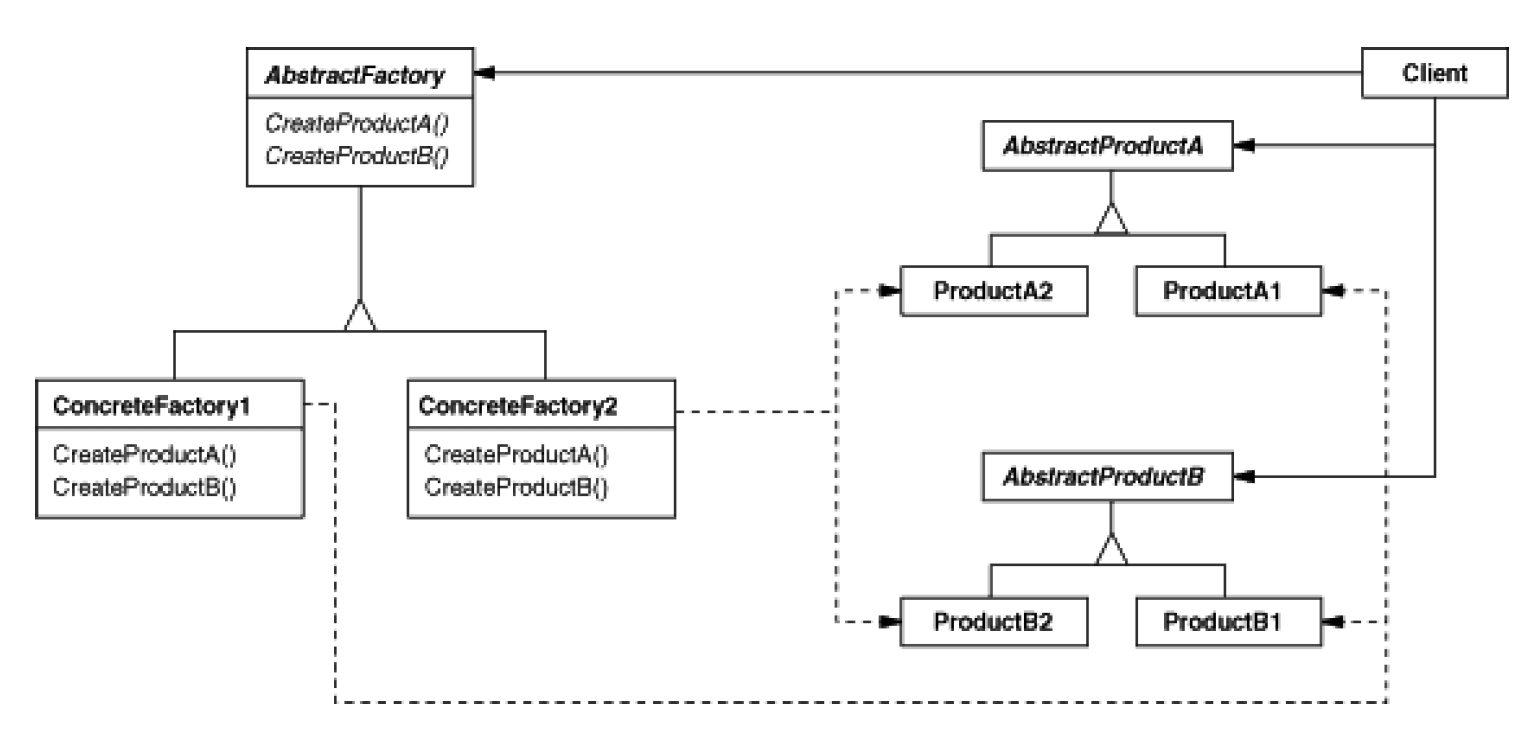
\includegraphics[scale=0.5]{structure.png}
\end{center}
\end{frame}
%-------------------------------------------------------------------------------------------------

\subsection{Հետևանքները}
%-------------------------------------------------------------------------------------------------
\begin{frame}\frametitle{Հետևանքները}
Այս Ն.Ձ. ունի հետևյալ առավելություններն ու թերությունները.
\vfill
\begin{enumerate}
    \item Վերահսկվող դիմում միակ օրինակին: \pause \vfill
    \item Կրճատված անվանային տարածություն: \pause \vfill
    \item Գործողությունների և իրականացման լավացման հնարավորություն: \pause \vfill
    \item Գոյություն ունեցող օրինակների մաքսիմալ քանակի` կամայական
    ֆիքսված թվով սահմանափակման հնարավորություն (Multiton pattern): \pause \vfill
    \item Ավելի ճկուն քան static ֆունկցիաների միջոցով իրականացումը:
\end{enumerate}
\end{frame}
%-------------------------------------------------------------------------------------------------

\section{Իրականացումը}
%-------------------------------------------------------------------------------------------------
\begin{frame}\frametitle{Իրականացումը}
\begin{enumerate}
    \item Օբյեկտի միակության ապահովում:
\end{enumerate}
\end{frame}
%-------------------------------------------------------------------------------------------------

%-------------------------------------------------------------------------------------------------
\begin{frame}[fragile]\frametitle{Դասական Իրականացում}
\begin{english}
\begin{minted}[fontsize=\scriptsize]{cpp}
class Singleton {

public:
    static Singleton* Instance();

protected:
    Singleton();

private:
    static Singleton* instance;
};

Singleton* Singleton::instance = NULL;

Singleton* Singleton::Instance() {
    if (instance == 0) {
        instance = new Singleton;
    }
    return instance;
}
\end{minted}
\end{english}
\end{frame}
%-------------------------------------------------------------------------------------------------

%-------------------------------------------------------------------------------------------------
\begin{frame}[fragile]\frametitle{Սխալ Իրականացում}
\begin{english}
\begin{minted}{cpp}
class Singleton {

public:
    static Singleton* Instance();

protected:
    Singleton();

private:
    static Singleton instance;
};

Singleton Singleton::instance;

Singleton* Singleton::Instance() {
    return &instance;
}
\end{minted}
\end{english}
\end{frame}
%-------------------------------------------------------------------------------------------------

%-------------------------------------------------------------------------------------------------
\begin{frame}[fragile]\frametitle{Meyers' Singleton}
\begin{english}
\begin{minted}{cpp}
static Singleton& Singleton::Instance()
{
    static Singleton instance;
    return instance;
}
\end{minted}
\end{english}
\end{frame}
%-------------------------------------------------------------------------------------------------

%-------------------------------------------------------------------------------------------------
\begin{frame}\frametitle{Իրականացումը}
\begin{enumerate}
    \item Օբյեկտի միակության ապահովում: \vfill
    \item Մեկից ավել փոխհամագործակցող Singleton դասերի առկայության
    դեպքում նրանց ոչնչացման հերթականության ղեկավարում: \vfill
    \item Singleton դասից ժառանգում:
\end{enumerate}
\end{frame}
%-------------------------------------------------------------------------------------------------

%-------------------------------------------------------------------------------------------------
\begin{frame}[fragile]\frametitle{Լավացված Իրականացում}
\begin{english}
\begin{minted}{cpp}
class Singleton {

public:
    static Singleton& Instance();

protected:
    Singleton();
    ~Singleton();

private:
    Singleton(const Singleton &) = delete;
    Singleton(Singleton &&) = delete;
    Singleton& operator=(const Singleton &) = delete;
    Singleton& operator=(Singleton &&) = delete;
};
\end{minted}
\end{english}
\end{frame}
%-------------------------------------------------------------------------------------------------

%-------------------------------------------------------------------------------------------------
\begin{frame}[fragile]\frametitle{Singleton Դասից Ժառանգում}
\begin{english}
\begin{minted}{cpp}
class Singleton {

public:
    static void Register(const char* name, Singleton*);
    static Singleton* Instance();

protected:
    static Singleton* Lookup(const char* name);

private:
    static Singleton* instance;
    static List<NameSingletonPair>* registry;
};
\end{minted}
\end{english}
\end{frame}
%-------------------------------------------------------------------------------------------------

%-------------------------------------------------------------------------------------------------
\begin{frame}[fragile]\frametitle{Singleton Դասից Ժառանգում}
\begin{english}
\begin{minted}{cpp}
Singleton* Singleton::Instance() {
    if (instance == 0) {
        const char* singletonName = getenv("SINGLETON");
        instance = Lookup(singletonName);
    }
    return instance;
}

MySingleton::MySingleton() {
    Singleton::Register("MySingleton", this);
}
\end{minted}
\end{english}
\end{frame}
%-------------------------------------------------------------------------------------------------

%-------------------------------------------------------------------------------------------------
\begin{frame}\frametitle{Իրականացումը}
\begin{enumerate}
    \item Օբյեկտի միակության ապահովում: \vfill
    \item Մեկից ավել փոխհամագործակցող Singleton դասերի առկայության
    դեպքում նրանց ոչնչացման հերթականության ղեկավարում: \vfill
    \item Singleton դասից ժառանգում: \vfill
    \item Thread Safety
\end{enumerate}
\end{frame}
%-------------------------------------------------------------------------------------------------

%-------------------------------------------------------------------------------------------------
\begin{frame}[fragile]\frametitle{Դասական Իրականացում}
\begin{english}
\begin{minted}{cpp}
Singleton* Singleton::Instance () {
    if (instance == 0)  {         // 1
        instance = new Singleton; // 2
    }
    return instance;              // 3
}
\end{minted}
\end{english}
\end{frame}
%-------------------------------------------------------------------------------------------------

%-------------------------------------------------------------------------------------------------
\begin{frame}[fragile]\frametitle{Thread Safety}
\begin{english}
\begin{minted}{cpp}
Singleton* Singleton::Instance () {
    Lock guard(mutex);
    if (instance == 0)  {         // 1
        instance = new Singleton; // 2
    }
    return instance;              // 3
}
\end{minted}
\end{english}
\end{frame}
%-------------------------------------------------------------------------------------------------

%-------------------------------------------------------------------------------------------------
\begin{frame}[fragile]\frametitle{Thread Safety – Սխալ Լուծում}
\begin{english}
\begin{minted}{cpp}
Singleton* Singleton::Instance () {
    if (instance == 0)  {         // 1
        Lock guard(mutex);        // 2
        instance = new Singleton; // 3
    }
    return instance;              // 4
}
\end{minted}
\end{english}
\end{frame}
%-------------------------------------------------------------------------------------------------

%-------------------------------------------------------------------------------------------------
\begin{frame}[fragile]\frametitle{Thread Safety – Մասամբ Ճիշտ Լուծում}
\begin{english}
\begin{minted}{cpp}
Singleton* Singleton::Instance () {
    if (instance == 0) {               // 1
        Lock guard(mutex);             // 2
        if (instance == 0) {           // 3
            instance = new Singleton;  // 4
        }
    }
    return instance;                   // 5
}
\end{minted}
\end{english}
\end{frame}
%-------------------------------------------------------------------------------------------------

%-------------------------------------------------------------------------------------------------
\begin{frame}[fragile]\frametitle{Thread Safety Java-ում}
\begin{english}
\begin{minted}[fontsize=\scriptsize]{java}
public class Singleton {

    private static Singleton uniqueInstance;

    private Singleton() {}

    /**
     * By adding the synchronized keyword to getInstance(), we force
     * every thread to wait its turn before it can enter the method.
     * That is, no two threads may enter the method at the same time.
     */
    public static synchronized Singleton getInstance() {

        if (uniqueInstance == null) {
            uniqueInstance = new Singleton();
        }
        return uniqueInstance;
    }
}
\end{minted}
\end{english}
\end{frame}
%-------------------------------------------------------------------------------------------------

%-------------------------------------------------------------------------------------------------
\begin{frame}[fragile]\frametitle{Thread Safety Java-ում}
\begin{english}
\begin{minted}[fontsize=\scriptsize]{java}
public class Singleton {

    /**
     * Creating an instance in a static initializer
     * This code is guaranteed to be thread safe!
     */
    private static Singleton uniqueInstance = new Singleton();

    private Singleton() {}

    public static Singleton getInstance() {

        // We already have an instance, so just return it
        return uniqueInstance;
    }
}
\end{minted}
\end{english}
\end{frame}
%-------------------------------------------------------------------------------------------------

%-------------------------------------------------------------------------------------------------
\begin{frame}[fragile]\frametitle{Thread Safety Java-ում}
\begin{english}
\begin{minted}[fontsize=\tiny]{java}
public class Singleton {

    /**
     * The volatile keyword ensures that multiple threads handle the uniqueInstance
     * variable correctly when it is being initialized to the Singleton instance.
     */
    private volatile static Singleton uniqueInstance;

    private Singleton() {}

    public static Singleton getInstance() {

        // If there is no instance, enter a synchronized block
        if (uniqueInstance == null) {

            // Note we only synchronize the first time through!
            synchronized (Singleton.class) {

                // Check again and if still null, create an instance
                if (uniqueInstance == null) {

                    uniqueInstance = new Singleton();
                }
            }
        }
        return uniqueInstance;
    }
}
\end{minted}
\end{english}
\end{frame}
%-------------------------------------------------------------------------------------------------

%-------------------------------------------------------------------------------------------------
\begin{frame}[fragile]\frametitle{Thread Safety Bill Pugh-ի Լուծում}
\begin{english}
\begin{minted}[fontsize=\scriptsize]{java}
public class Singleton {

    private Singleton() { }

    /**
     * SingletonHolder is thread safely loaded on the first access to
     * SingletonHolder.instance which is the first call of getInstance
     */
    private static class SingletonHolder {
        public static final Singleton instance = new Singleton();
    }

    public static Singleton getInstance() {
        return SingletonHolder.instance;
    }
}
\end{minted}
\end{english}
\end{frame}
%-------------------------------------------------------------------------------------------------

\subsection{Օրինակ}
%-------------------------------------------------------------------------------------------------
\begin{frame}[fragile]\frametitle{Օրինակ}
\begin{english}
\begin{minted}{cpp}
class MazeFactory {

public:
    static MazeFactory* Instance();

    // existing interface goes here

protected:
    MazeFactory();

private:
    static MazeFactory* instance;
};
\end{minted}
\end{english}
\end{frame}
%-------------------------------------------------------------------------------------------------

%-------------------------------------------------------------------------------------------------
\begin{frame}[fragile]\frametitle{Օրինակ}
\begin{english}
\begin{minted}{cpp}
MazeFactory* MazeFactory::instance = 0;

MazeFactory* MazeFactory::Instance() {

    if (instance == 0) {
        instance = new MazeFactory;
    }
    return instance;
}
\end{minted}
\end{english}
\end{frame}
%-------------------------------------------------------------------------------------------------

%-------------------------------------------------------------------------------------------------
\begin{frame}[fragile]\frametitle{Օրինակ}
\begin{english}
\begin{minted}[fontsize=\scriptsize]{cpp}
MazeFactory* MazeFactory::instance = 0;

MazeFactory* MazeFactory::Instance () {
    if (instance == 0) {
        const char* mazeStyle = getenv("MAZESTYLE");

        if (strcmp(mazeStyle, "bombed") == 0) {
            instance = new BombedMazeFactory;

        } else if (strcmp(mazeStyle, "enchanted") == 0) {
            instance = new EnchantedMazeFactory;

        } else {
            instance = new MazeFactory; // default
        }
    }
    return instance;
}
\end{minted}
\end{english}
\end{frame}
%-------------------------------------------------------------------------------------------------

\section{Առնչվող Ձևանմուշները}
%-------------------------------------------------------------------------------------------------
\begin{frame}\frametitle{Առնչվող Նախագծման Ձևանմուշները}
\begin{itemize}
    \item Abstract Factory \vfill
    \item Facade \vfill
    \item Observer \vfill
    \item State
\end{itemize}
\end{frame}
%-------------------------------------------------------------------------------------------------

\end{document}
